%
% Reading the Eyes, Not the Mind? -- Ocular-Confound Auditor for EEG decoding
% Two-column layout (matching the supplied "double-bar" template).
%
% Compile with:
%   tectonic manuscript.tex          (runs LaTeX + bibtex automatically)
% or:
%   pdflatex manuscript ; bibtex manuscript ; pdflatex manuscript ; pdflatex manuscript
%
% Required files in the same directory:
%   sn-bibliography.bib, unsrtnat.bst,
%   fig1_montage.png fig2_topographies.png fig3_h3_battery.png fig4_coupling.png
%   fig5_bias_envelope.png fig6_reliability_gate.png fig7_real_eegmmidb.png fig8_leakage_angle.png
%

\documentclass[10pt,twocolumn]{article}

%%%% Packages
\usepackage[margin=1in]{geometry}
\usepackage{graphicx}
\usepackage{amsmath,amssymb}
\usepackage{booktabs}
\usepackage{array}
\usepackage{tabularx}
\usepackage{setspace}
\usepackage{url}
\usepackage[numbers,sort&compress]{natbib}
\usepackage{hyperref}
\usepackage{threeparttable}
\usepackage{caption}
\usepackage{titlesec}

%%%% Two-column typography (matches the template look)
\captionsetup{font=small, labelfont=bf}
\setlength{\parindent}{1.5em}
\setlength{\columnsep}{0.30in}
\setlength{\parskip}{0pt}
\setlength{\textfloatsep}{12pt plus 2pt minus 2pt}

\titleformat{\section}{\normalfont\large\bfseries}{\thesection}{0.6em}{}
\titleformat{\subsection}{\normalfont\normalsize\bfseries}{\thesubsection}{0.5em}{}
\titleformat{\subsubsection}{\normalfont\normalsize\itshape}{\thesubsubsection}{0.5em}{}
\titlespacing*{\section}{0pt}{1.4ex plus .2ex}{0.8ex}
\titlespacing*{\subsection}{0pt}{1.1ex plus .2ex}{0.6ex}

\begin{document}

\singlespacing

%%──────────────────────────────────────────────────────────
%% TITLE PAGE
%%──────────────────────────────────────────────────────────

\twocolumn[{%
\begin{center}
{\LARGE\bfseries Reading the Eyes, Not the Mind? A Portable, Montage-Matched Auditor for Ocular Confounds in EEG Decoding\par}

\vspace{1.2em}

% Authors intentionally left blank.
{\large \strut \par}

\vspace{0.6em}

% Affiliations intentionally left blank.
{\small \strut}

\vspace{0.8em}

{\small\textbf{Corresponding author:} \rule[-0.4ex]{4cm}{0.4pt}}
\end{center}

\vspace{0.8em}

%%──────────────────────────────────────────────────────────
%% ABSTRACT
%%──────────────────────────────────────────────────────────

\begin{center}
\textbf{\large Abstract}
\end{center}
\begin{quote}
\small
\textbf{Background:} Eye movements, blinks, and the corneo-retinal standing potential leak
into scalp electroencephalography (EEG) and co-vary with task structure, so a classifier
that claims to decode a cognitive state may instead be partly reading the eyes. Existing
defenses either \emph{remove} ocular signal or model it within a single eye-tracked
recording; none provides a portable measurement of how much of a published decoding result
could be ocular, for the many datasets recorded without an eye-tracker.
\textbf{Methods:} We define and validate an auditing instrument. A frozen linear EEG-to-gaze
readout, trained where synchronized gaze exists, induces a locked \emph{ocular subspace}
(the orthogonal projection onto the span of its weights). The auditor operates on \emph{all}
available channels: we report a full 64-channel montage and, as an explicitly specified
subset, the 30-channel ERP-CORE set. The \emph{Ocular Predictability Index} (OPI) is the
cross-validated area under the curve (AUC) of a paradigm-matched decoder applied to that
projection, minus a within-subject label-permutation null. The instrument ships with a
three-tier reliability gate that returns ``inconclusive'' when gaze cannot be reconstructed
in the target montage, a measured two-sided bias envelope, and a computable neural-leakage
bound. Drawing montage and physiological parameters from several public datasets (EEGEyeNet,
ERP CORE, and the electrooculography literature), we validate against ground truth in a
physically grounded EEG+gaze simulator and on real 64-channel EEG (PhysioNet
\texttt{eegmmidb}).
\textbf{Results:} The OPI is 0.43 on saccade-coupled ocular data and 0.20 on a
condition-correlated eye-blink artifact (a distinct artifact type), versus $\le$0.03 on every
negative control (covert attention, motor imagery, label shuffle), rising monotonically with
the artifact--label coupling. A lateralized neural source decodable from full EEG (AUC 0.79)
is not decodable from the ocular projection (OPI 0.007, n.s.). The auditor's index matches the
ground-truth-gaze index to within $\pm$0.01 except, conservatively, at the fixational extreme
on the sparse montage. Neural leakage is governed by the principal-angle overlap between the
cognitive topography and the ocular subspace (Spearman $\rho=0.95$; leakage $\approx 0$ for a
posterior source). On real EEG, a left-versus-right motor-imagery contrast yields OPI
$-0.023$ ($p=0.998$). \textbf{Conclusions:} A frozen, montage-matched ocular-subspace
auditor turns ``how much of this is the eyes?'' into a calibrated, two-sided number with a
self-declared competence boundary, enabling portable ocular-leakage audits of EEG decoding
results recorded without an eye-tracker.

\vspace{0.5em}

\noindent\textbf{Keywords:} EEG decoding; ocular artifact; eye movements; construct validity;
confound auditing; brain--computer interface; subspace projection
\end{quote}
\vspace{1.0em}
}]

%%──────────────────────────────────────────────────────────
%% BACKGROUND
%%──────────────────────────────────────────────────────────

\section{Background}

A decoding result is only as trustworthy as the signal it rests on. In EEG, a recurring
threat to construct validity is that a classifier credited with reading a cognitive
state---attention, working-memory load, target detection, the meaning of a read
word---is partly reading the eyes. The eye is an electrical dipole, cornea-positive and
retina-negative, with a standing potential of roughly $0.4$--$1.0$\,mV~\cite{malmivuo1995bioelectromagnetism};
its rotations, together with blinks and the broadband saccadic spike potential at saccade
onset~\cite{keren2010saccadic}, project to frontal and periocular electrodes with amplitudes
that dwarf cortical signals (Fig.~\ref{fig:efield}). Crucially, the field of an eye movement
depends on each electrode's \emph{position} relative to the eyes---its sign reverses across the
midline (a dipole) and its magnitude falls with distance---and a blink imposes a different,
symmetric pattern, so the contamination an electrode sees is montage- and artifact-specific.
Because where and when a person looks is rarely independent of the experimental condition,
this ocular activity is \emph{condition-correlated}: it can be decoded in lockstep with the
cognitive label and inflate apparent accuracy. The danger is the machine-learning failure
mode of shortcut learning---exploiting an incidental correlate rather than the intended
construct~\cite{geirhos2020shortcut}.

\begin{figure*}[tb]
\centering
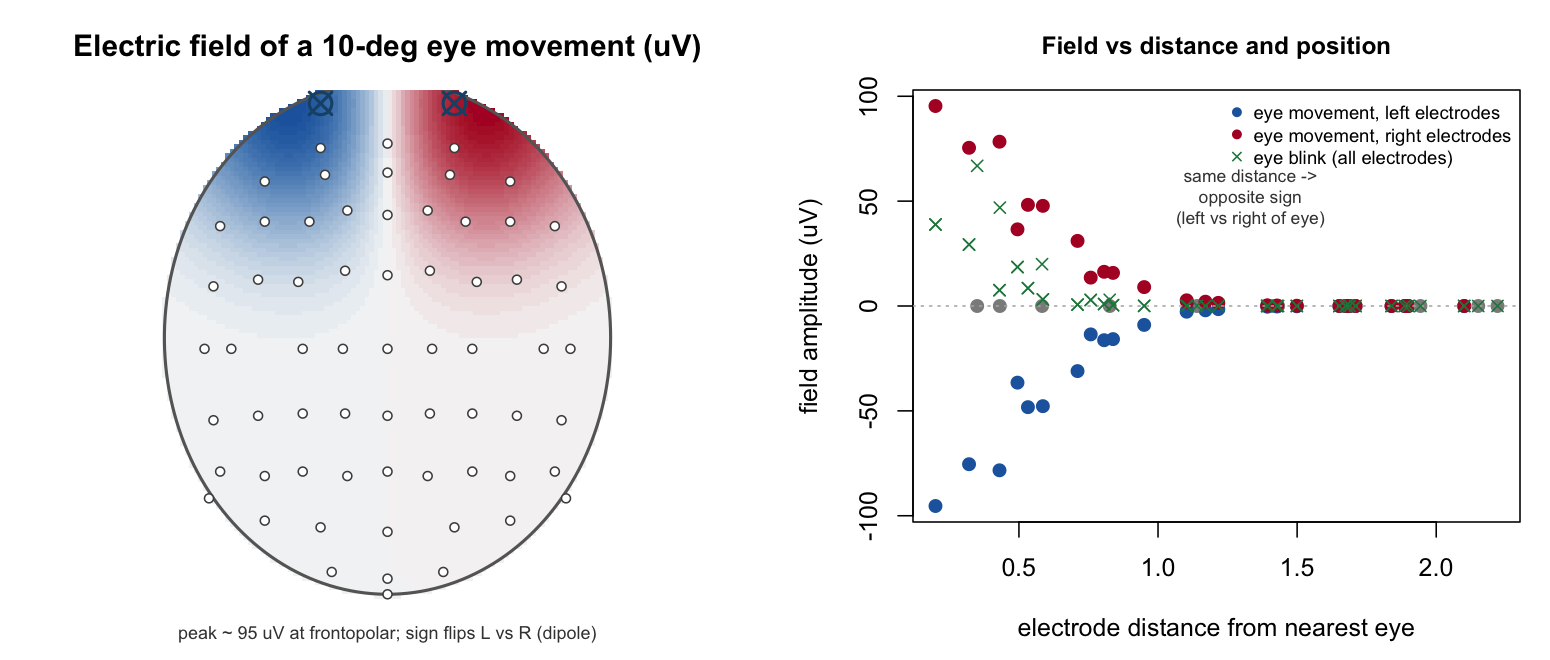
\includegraphics[width=0.95\textwidth]{fig9_efield.png}
\caption{The electric field of an eye movement depends on electrode position. \emph{Left:}
scalp field of a $10^\circ$ horizontal eye movement over the 64-channel montage (peak
$\approx 95\,\mu$V at frontopolar sites; sign reverses left/right of the eyes---a dipole).
\emph{Right:} field amplitude versus each electrode's distance from the nearest eye. At a given
distance the sign depends on which side of the eyes the electrode sits (blue vs.\ red); an eye
blink (green) imposes a distinct, symmetric, one-signed field that also decays with distance.
This position- and artifact-dependence is why the auditor is montage-matched.}\label{fig:efield}
\end{figure*}

The standard defenses are incomplete. Independent component analysis and regression
\emph{remove} ocular components~\cite{jung2000removing,plochl2012combining}, but removal is
imperfect and leaves a residual whose decodable content is unknown; overweighting the
saccadic spike before ICA improves this but still targets removal, not
measurement~\cite{dimigen2020optimizing,piontonachini2019iclabel}. Deconvolution frameworks
rigorously model ocular and overlap effects, but in practice within a single, carefully
co-registered, eye-tracked recording~\cite{ehinger2019unfold,dimigen2011coregistration}.
None of these answers the question an author or a reviewer actually faces about a finished
result: \emph{what fraction of this decodable signal could be ocular?}---particularly for the
thousands of datasets recorded with no eye-tracker at all.

The concern is not hypothetical. \citet{mostert2018eye} showed that a visual working-memory
``representation'' could be partly explained by systematic eye movements, and constructed a
bespoke, within-experiment control: if the target variable cannot be decoded from
simultaneously recorded gaze, the neural result is safer. \citet{rotaru2024decoding} found
that EEG decoders of the spatial focus of \emph{auditory} attention overfit to eye-gaze and
per-trial fingerprints, dropping to chance once gaze was controlled. More broadly, the
neuroimaging and machine-learning literatures increasingly reward auditing the field's
methods and benchmarks for inflated inference---cluster-extent false positives in
fMRI~\cite{eklund2016cluster}, pervasive data leakage in ML-based
science~\cite{kapoor2023leakage} and specifically in deep-learning
EEG~\cite{brookshire2024leakage}, and permutation-based tests for
confounding~\cite{chaibubneto2018permutations}. What is missing is a \emph{transferable
instrument}: a frozen, montage-matched ocular-subspace probe that can be pointed at an
arbitrary EEG decoding dataset---including one with no gaze recording---and that returns a
calibrated number together with an honest statement of when it cannot be trusted.

This paper defines and validates that instrument. Our contributions are: (i) a locked,
linear ocular-subspace operator and an \emph{Ocular Predictability Index} (OPI) with a
within-subject permutation null and a full-EEG ceiling; (ii) a three-tier reliability gate
that returns ``inconclusive'' rather than a false clean bill of health; (iii) a \emph{measured}
two-sided bias envelope, so the index can neither silently hide contamination nor over-blame
the eyes; and (iv) a \emph{computable neural-leakage bound}---the one residual failure mode,
that the projection absorbs genuine neural signal, is shown to be governed by the principal
angle between the cognitive topography and the ocular subspace, converting a reviewer's
objection into a number. We validate all four against ground truth in a physically grounded
simulator and demonstrate the instrument on real 64-channel EEG.

%%──────────────────────────────────────────────────────────
%% METHODS
%%──────────────────────────────────────────────────────────

\section{Methods}

\subsection{Design and rationale}

The instrument is deliberately linear. Although a deep network is one way to learn an
EEG-to-gaze readout where synchronized eye-tracking is
available~\cite{kastrati2021eegeyenet,hollenstein2018zuco}, the object that is frozen and
shipped is a linear readout and the orthogonal projection onto the span of its weights. We
therefore implement and validate exactly that object. Because ground truth---knowing how much
of a decodable signal is truly ocular---is available only when gaze is recorded or simulated,
the primary validation uses a forward-model simulator with known sources, complemented by a
real-EEG negative control.

The auditor uses \emph{every} channel a dataset provides; dimensionality is never silently
reduced. We report a full 64-channel 10--10 montage as primary and treat the 30-channel
ERP-CORE set as an \emph{explicitly specified subset} of it, used only to characterise how
channel count and near-eye frontal coverage affect the auditor (the reliability gate, below).
Validation draws on more than one dataset: EEGEyeNet---hundreds of subjects with 128-channel
EEG and synchronized eye-tracking---is the source paradigm and montage family from which the
gaze readout would be trained~\cite{kastrati2021eegeyenet}; ERP CORE supplies the 30-channel
target montage~\cite{kappenman2021erpcore}; PhysioNet \texttt{eegmmidb} supplies real
64-channel EEG~\cite{schalk2004bci2000}; and ZuCo provides a same-cap-family reading corpus for
the near-fixation regime~\cite{hollenstein2018zuco}. Source amplitudes are taken from the
electrooculography and saccade literature.

\subsection{The locked ocular-subspace operator}

Let $\mathbf{X}_{\mathrm{src}}\in\mathbb{R}^{n\times p}$ be source EEG (trials $\times$
channels) for which ocular ground truth $\mathbf{Y}_{\mathrm{src}}\in\mathbb{R}^{n\times q}$
is available ($q$ outputs: horizontal and vertical gaze, a saccade channel, and a blink
indicator). A ridge readout
$\mathbf{W}=\arg\min_{\mathbf W}\lVert \mathbf{Y}_{\mathrm{src}}-\mathbf{X}_{\mathrm{src}}\mathbf{W}\rVert_F^2+\lambda\lVert\mathbf{W}\rVert_F^2$
maps EEG to ocular state. The \emph{ocular subspace} is the column space of $\mathbf{W}$, and
the locked operator is the orthogonal projection onto it,
\begin{equation}
\mathbf{P}=\mathbf{U}\mathbf{U}^{\top},\qquad \mathbf{U}=\text{left singular vectors of }\mathbf{W},
\label{eq:proj}
\end{equation}
a symmetric idempotent $p\times p$ matrix ($\mathbf{P}^2=\mathbf{P}$). Projecting target EEG,
$\mathbf{X}\mapsto\mathbf{X}\mathbf{P}$, retains only the component lying in the ocular
readout's span. The operator is fixed by Eq.~\eqref{eq:proj} before any audit; the auditor is
retrained on each target's exact channel set (montage-matched, no interpolation of periocular
channels).

\subsection{The Ocular Predictability Index}

A paradigm-matched cognitive decoder (a ridge linear classifier) is trained and tested under
strictly subject-wise cross-validation on the projected data $\mathbf{X}\mathbf{P}$, yielding a
macro-averaged AUC. The OPI subtracts a within-subject label-permutation null (labels shuffled
within each subject, $B=200$):
\begin{equation}
\mathrm{OPI}=\mathrm{AUC}_{\mathrm{proj}}-\overline{\mathrm{AUC}}_{\mathrm{null}},
\end{equation}
and is reported alongside the full-EEG AUC as a ceiling and a permutation $p$-value. The
auditor never sees the target cognitive labels, so audits are out-of-distribution by
construction.

\subsection{Reliability gate and bias envelope}

\emph{Reliability} is the cross-validated gaze-reconstruction $R^2$ of the montage-restricted
readout, a property of the montage that requires no target eye-tracker. Thresholds are derived
empirically from the relationship between reliability and index bias and partition results into
\emph{confirmatory}, \emph{exploratory}, and \emph{inconclusive} tiers. The \emph{bias envelope}
is measured, not assumed: where ground-truth gaze exists, we compare the auditor's OPI to the
OPI computed directly from true gaze across the saccade-amplitude range and report the signed
deviation as a two-sided margin.

\subsection{The neural-leakage bound}

The instrument's central risk is that the projection absorbs genuine neural activity that
happens to be gaze-correlated, inflating the index. We bound this. For a target whose cognitive
decoder has contrast topography $\mathbf{t}$, define the overlap
\begin{equation}
s=\frac{\lVert\mathbf{P}\mathbf{t}\rVert}{\lVert\mathbf{t}\rVert}=\cos\theta,
\label{eq:overlap}
\end{equation}
the cosine of the principal angle $\theta$ between $\mathbf{t}$ and the ocular subspace. $s$
upper-bounds the fraction of the neural topography that can enter the projection; under the
linear model, leakage $\to 0$ as $s\to 0$. We report $s$ per audit and test the predicted
monotonicity empirically.

\subsection{Grounded EEG+gaze simulator}

Ground-truth validation uses a forward-model simulator on a full 64-channel 10--10
montage; the 30 ERP-CORE electrodes~\cite{kappenman2021erpcore} are an explicitly labelled
subset of these 64 (Fig.~\ref{fig:montage}), so the auditor is exercised on all 64 channels and
the 30-channel case is a deliberately studied restriction, never a silent reduction. Per-trial
channel patterns are sums of physically grounded source topographies (Figs.~\ref{fig:efield},
\ref{fig:topo}): a horizontal corneo-retinal field ($\approx 16\,\mu$V per degree), a
vertical/blink frontopolar field, a focal periocular saccadic spike scaling with saccade
size~\cite{keren2010saccadic}, an $\approx 80\,\mu$V frontopolar blink, and a lateralized
posterior N2pc-like neural component ($\approx 1.8\,\mu$V)~\cite{luck1994n2pc}, on spatially
correlated background noise. An artifact is coupled to the cognitive label with tunable
strength, implementing the condition-correlated premise. Scenarios include saccade-coupled
ocular and \emph{blink-coupled} ocular (two positive controls testing distinct artifact types),
covert attention (lateralized posterior neural source, central gaze), focal motor imagery,
label shuffle, and a neutral baseline.

\subsection{Real data}

We use PhysioNet \texttt{eegmmidb} (all 64 channels, BCI2000, 160\,Hz, EDF+; 8
subjects)~\cite{schalk2004bci2000,goldberger2000physionet}; no channels are dropped. Because
\texttt{eegmmidb} has no eye-tracker, the ocular subspace is estimated from the eyes-open
baseline run of four \emph{source} subjects (a real-EEG analogue of a frozen gaze-trained
auditor) and applied to four held-out \emph{target} subjects' motor runs. We audit two
contrasts: left-versus-right imagined movement (no differential gaze expected; the clean
negative control) and rest-versus-movement.

\subsection{Implementation}

The auditor, simulator, and analyses are implemented in R (CPU-only). AUC is computed by the
rank statistic and cross-checked against the \texttt{pROC} package~\cite{robin2011proc} to
$<10^{-6}$. The trained auditor is small and CPU-deployable; code and results are released. The
deployment vision---applying the frozen instrument across public decoding benchmarks
(e.g.,~\cite{kappenman2021erpcore,gifford2022thingseeg2,arico2014p300jitter,korczowski2019bi2015a},
accessed via MOABB~\cite{jayaram2018moabb,tangermann2012bcicompetitioniv})---is discussed in
Section~\ref{sec:discussion}.

%%──────────────────────────────────────────────────────────
%% RESULTS
%%──────────────────────────────────────────────────────────

\section{Results}

\subsection{The operator behaves as specified}

Unit tests confirm the rank-based AUC matches \texttt{pROC} to $<10^{-6}$ including ties; the
projector of Eq.~\eqref{eq:proj} is symmetric and idempotent with the correct rank, fixes its
own column space, and annihilates the orthogonal complement; and, end-to-end, the OPI is large
and significant when the cognitive signal lies in the ocular subspace and non-significant when
it lies outside it. The trained auditors had ocular-subspace rank 4 (matching the four ocular
outputs) on the simulator montages and rank 2 on real \texttt{eegmmidb}.

\begin{figure*}[tb]
\centering
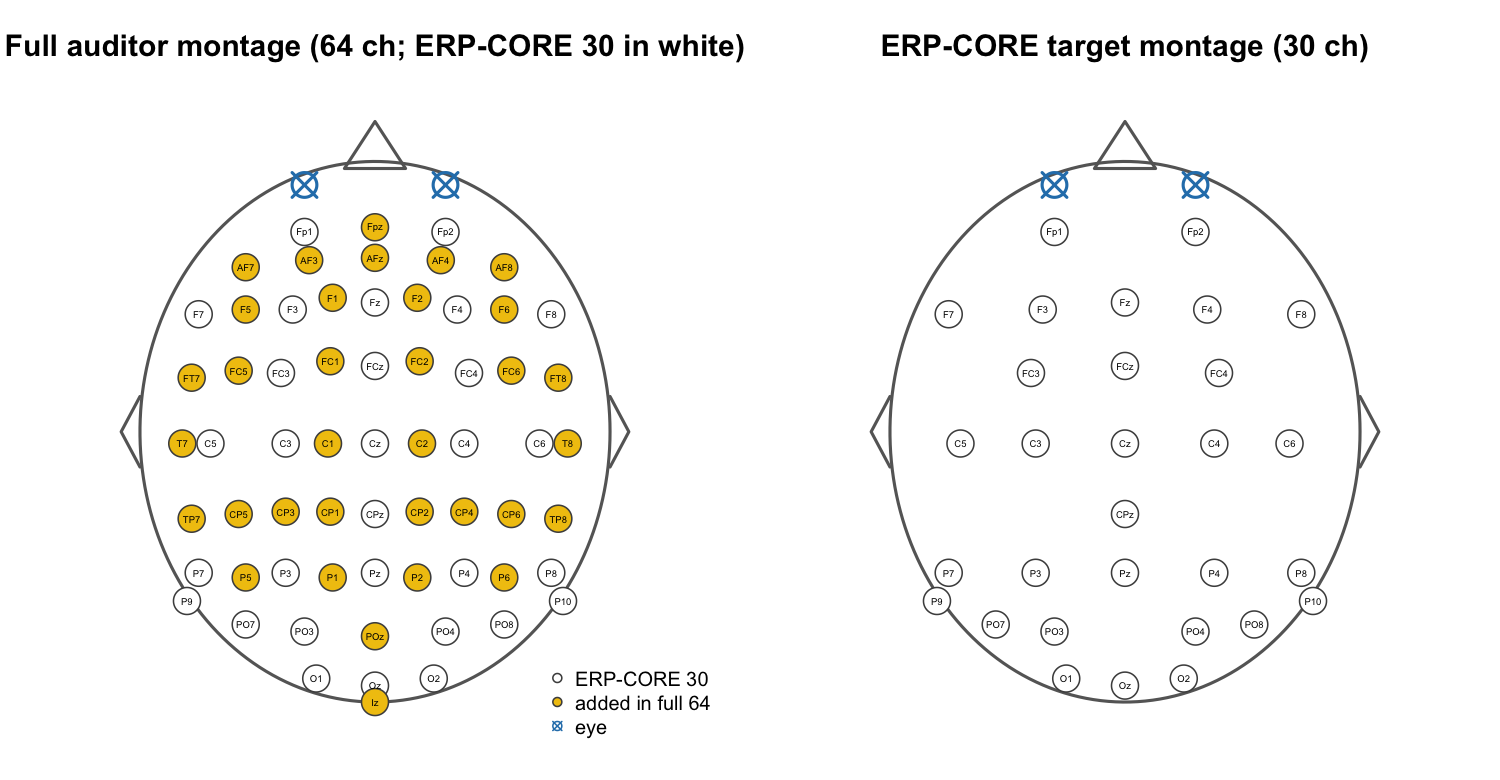
\includegraphics[width=0.92\textwidth]{fig1_montage.png}
\caption{Montages. The full auditor montage (left, 64 channels) contains the 30-channel
ERP-CORE set (white) plus 34 further 10--10 electrodes (yellow), including denser near-eye
frontal coverage that the 30-channel target montage (right) lacks; this density gap drives the
reliability gate. Eyes marked in blue.}\label{fig:montage}
\end{figure*}

\begin{figure*}[tb]
\centering
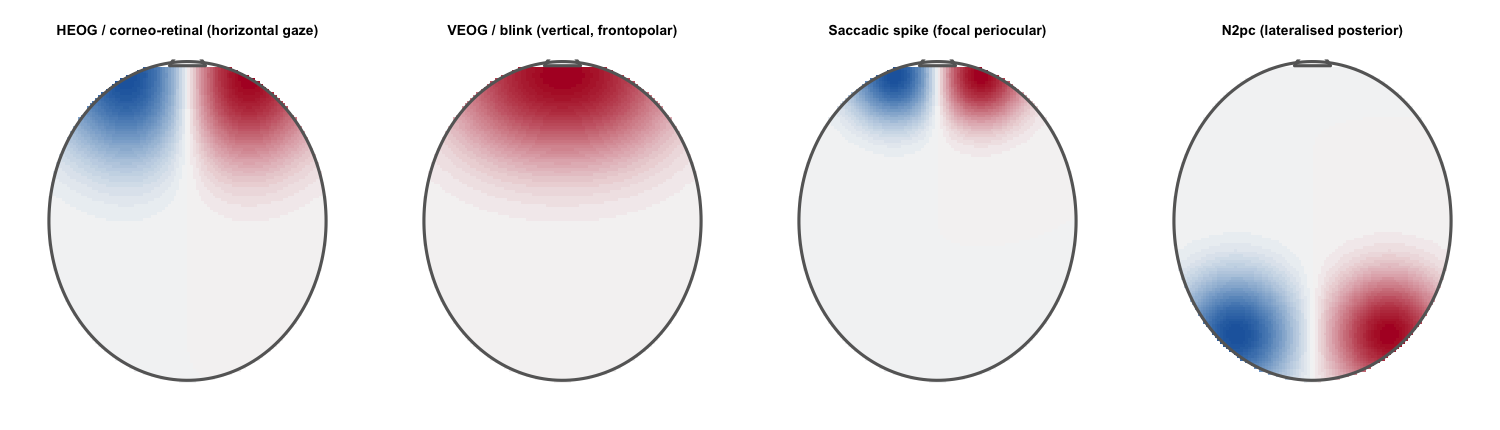
\includegraphics[width=0.92\textwidth]{fig2_topographies.png}
\caption{Physically grounded source topographies in the forward model: the antisymmetric
horizontal corneo-retinal (HEOG) field, the symmetric frontopolar vertical/blink field, the
focal periocular saccadic spike, and the lateralized posterior N2pc. Red/blue denote opposite
polarity.}\label{fig:topo}
\end{figure*}

\subsection{Graded sensitivity and specificity (H3)}

Across 12 independent simulated studies per cell on the full 64-channel montage, the OPI cleanly
separates ocular leakage from neural signal (Table~\ref{tab:battery}, Fig.~\ref{fig:battery}).
The two positive controls test \emph{distinct artifact types}: saccade-coupled ocular gives
OPI $=0.429$ with projected AUC equal to the full-EEG ceiling (0.929), and a condition-correlated
\emph{eye-blink} artifact gives OPI $=0.198$ (projected AUC 0.697)---both significant in 100\% of
studies. The auditor therefore detects blink contamination as well as saccade contamination.
Every negative control is near-null in magnitude: motor imagery 0.031, label-shuffle 0.007,
covert attention 0.007, neutral $-0.003$; their envelope sets an empirical \emph{calibrated
neural-leakage margin} of $\approx 0.05$ that the index must clear beyond the bare permutation
null. Decisively, the covert-attention contrast is decodable from full EEG (ceiling AUC 0.79)
yet not from the ocular projection (OPI 0.007, $p=0.48$): the auditor does not absorb lateralized
posterior neural signal.

\begin{table}[tb]
\centering
\caption{H3 sensitivity battery: the OPI separates ocular leakage from neural signal (mean of
12 simulated studies; full 64-channel montage).}\label{tab:battery}
\begin{threeparttable}
{\small
\begin{tabular*}{\columnwidth}{@{\extracolsep{\fill}} l cccc @{}}
\toprule
\textbf{Scenario} & \textbf{OPI} & \textbf{proj} & \textbf{ceiling} & \textbf{\% sig} \\
\midrule
Saccade-coupled ocular\tnote{a} & \textbf{0.429} & 0.929 & 0.930 & 100 \\
Blink-coupled ocular\tnote{a}   & \textbf{0.198} & 0.697 & 0.781 & 100 \\
Motor imagery          & 0.031 & 0.531 & 0.842 & 42 \\
Covert attention\tnote{b} & 0.007 & 0.507 & 0.785 & 17 \\
Label shuffle          & 0.007 & 0.507 & 0.505 & 0 \\
Neutral                & $-$0.003 & 0.496 & 0.635 & 0 \\
\bottomrule
\end{tabular*}}
\begin{tablenotes}
\small
\item proj $=$ AUC on the ocular projection; ceiling $=$ full-EEG AUC; \% sig $=$ studies with
permutation $p<0.05$.
\item[a] Positive control (two distinct artifact types). \item[b] Neural-leakage test:
decodable from full EEG, not from the ocular subspace.
\end{tablenotes}
\end{threeparttable}
\end{table}

\begin{figure}[tb]
\centering
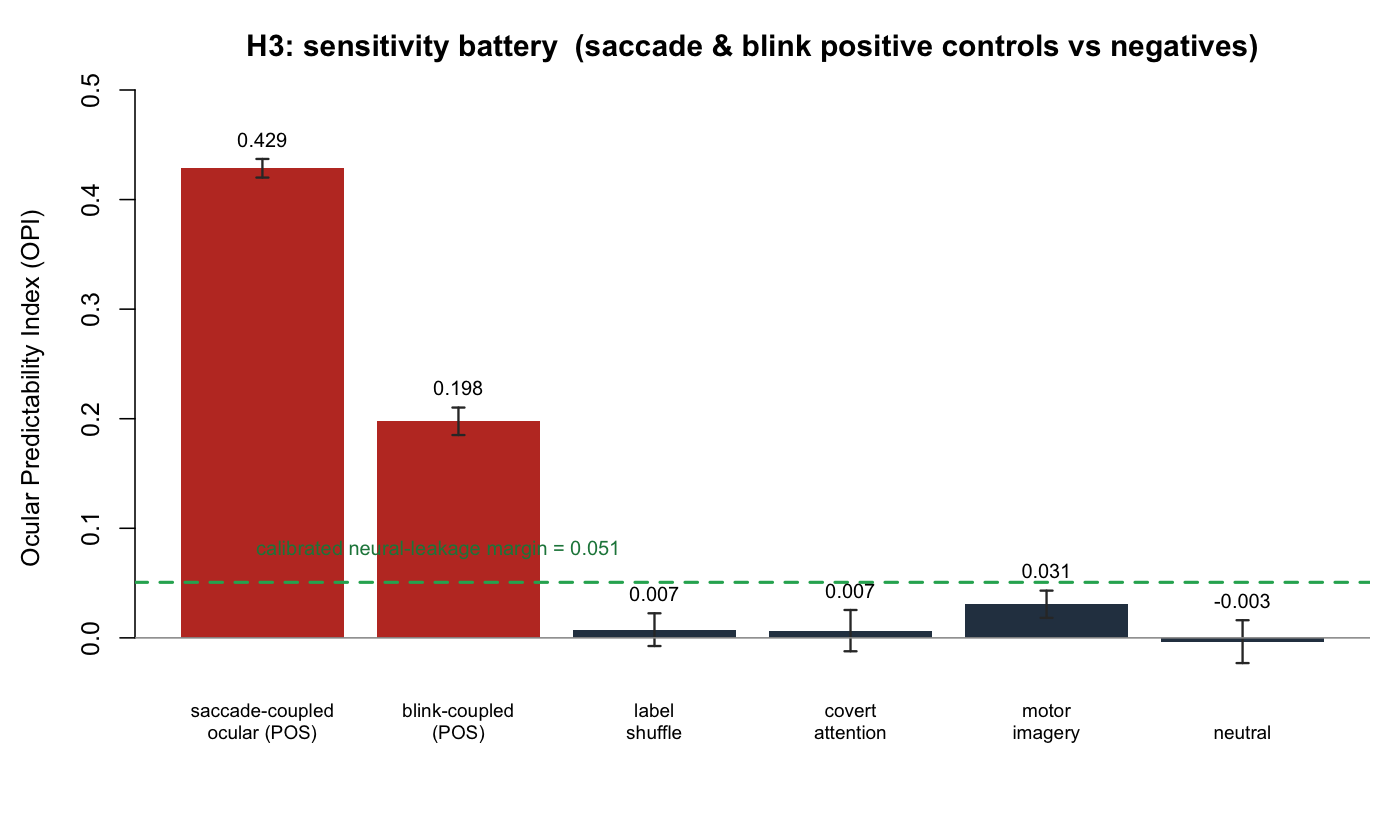
\includegraphics[width=\linewidth]{fig3_h3_battery.png}
\caption{H3 sensitivity battery. The two positive controls (red: saccade- and blink-coupled
ocular) exceed every negative control; all negative controls sit at or below the calibrated
neural-leakage margin (green dashed). Error bars are $\pm$SD over 12 studies.}\label{fig:battery}
\end{figure}

The index is a graded meter, not a binary flag: as the gaze--label coupling $\rho$ increases
from 0 to 1, the OPI rises monotonically and near-linearly from $-0.014$ to $0.500$, with the
projected AUC tracking from chance to 1.0 (Fig.~\ref{fig:coupling}).

\begin{figure}[tb]
\centering
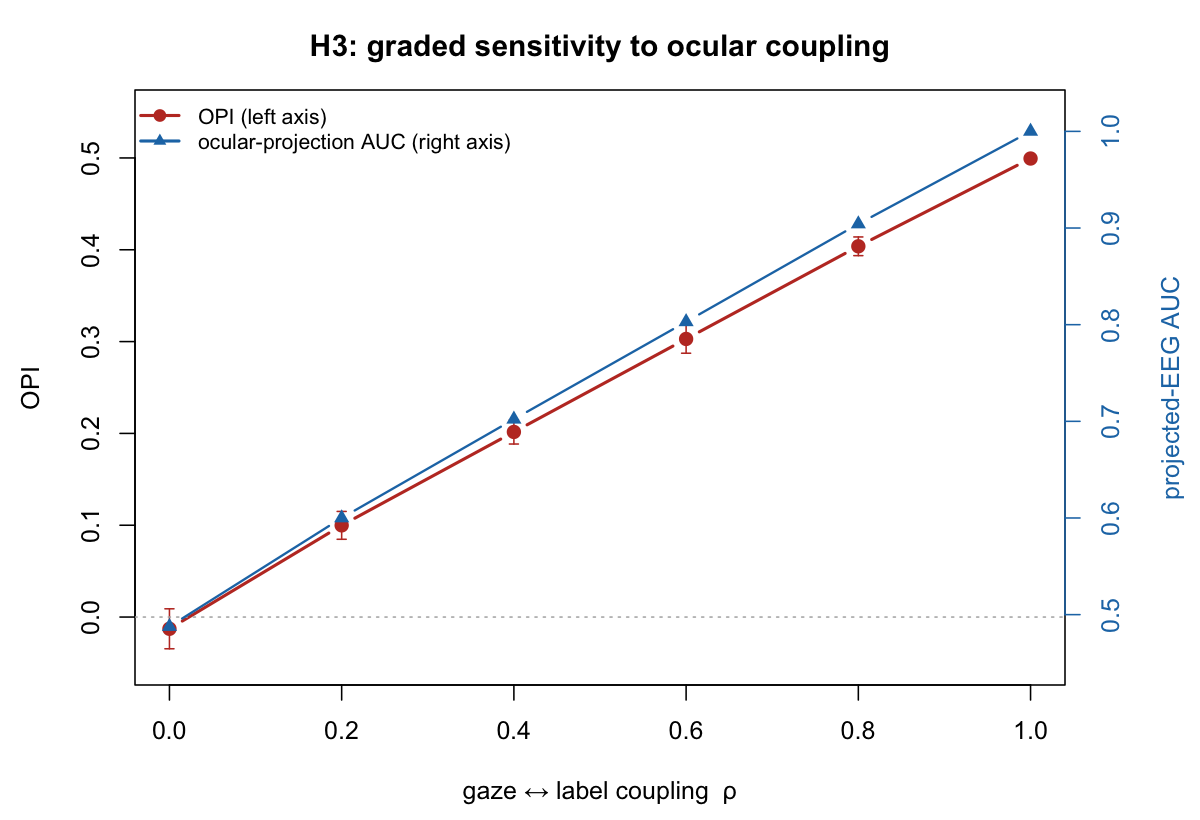
\includegraphics[width=\linewidth]{fig4_coupling.png}
\caption{Graded sensitivity: OPI (red, left axis) and ocular-projection AUC (blue, right axis)
rise monotonically with the gaze--label coupling.}\label{fig:coupling}
\end{figure}

\subsection{The bias envelope is conservative}

Comparing the auditor's OPI to the OPI from ground-truth gaze across the saccade-amplitude
range (Fig.~\ref{fig:bias}), the bias is within $\pm 0.01$ from $0.5^\circ$ upward on both
montages. Only at the fixational extreme ($0.25^\circ$) does it grow---to $-0.034$ on the full
64-channel montage and $-0.056$ on the 30-channel subset---and in both cases the auditor
\emph{under}-states the ocular contribution, the conservative direction. No over-statement was
observed. The breach magnitude is measured and folded into the trust tiers as a two-sided margin.

\begin{figure}[tb]
\centering
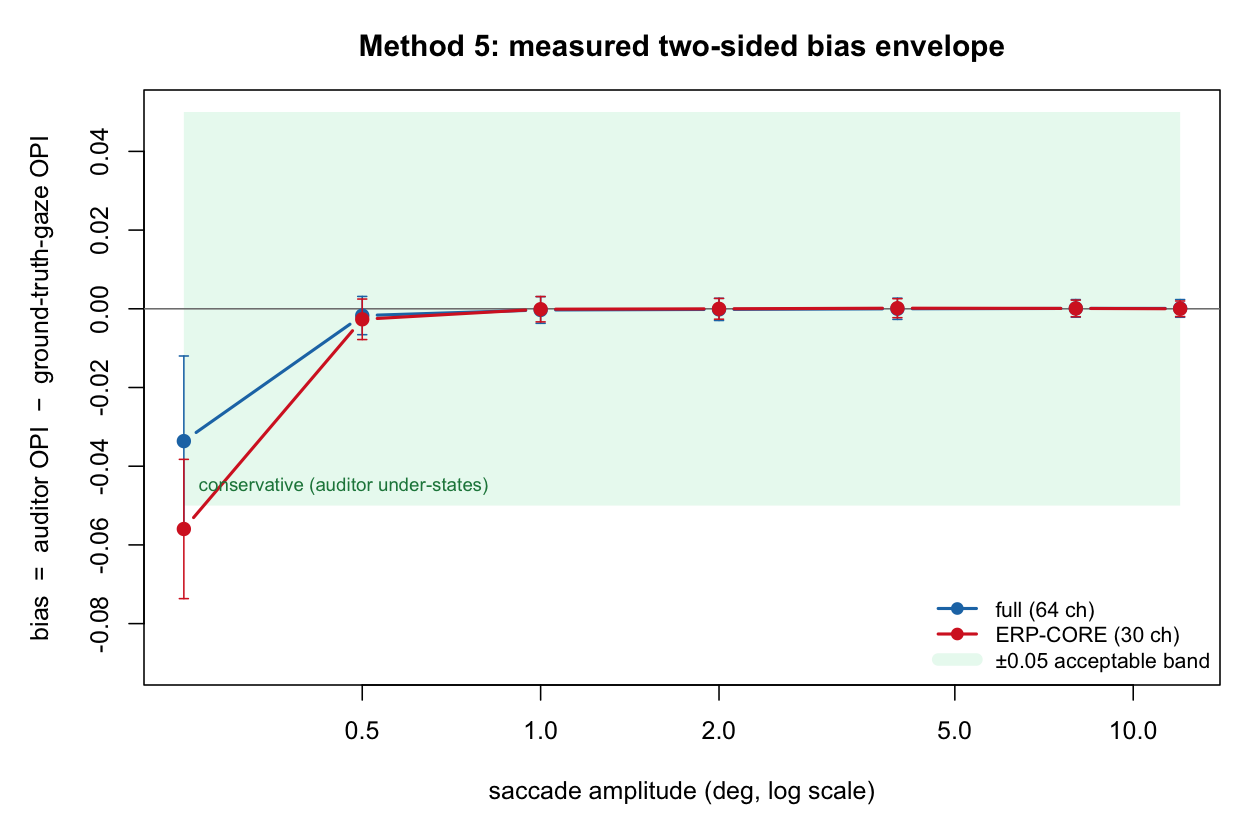
\includegraphics[width=\linewidth]{fig5_bias_envelope.png}
\caption{Measured two-sided bias envelope: auditor OPI minus ground-truth-gaze OPI versus
saccade amplitude. Deviations are negative (conservative) and confined to the fixational
extreme on the sparse montage.}\label{fig:bias}
\end{figure}

\subsection{The reliability gate has teeth}

The empirically calibrated thresholds are $R^2=0.664$ (confirmatory) and $R^2=0.497$
(exploratory). Tiering the amplitude $\times$ montage grid (Table~\ref{tab:reliab},
Fig.~\ref{fig:gate}), the full 64-channel montage is confirmatory at every amplitude, while the
30-channel subset falls to exploratory at the fixational extreme---precisely the regime
(sparse montage, sub-degree movement) where a silent failure would be most dangerous.

\begin{table}[tb]
\centering
\caption{Reliability ($R^2$), bias, and trust tier across saccade amplitude and montage.}\label{tab:reliab}
\begin{threeparttable}
{\small
\begin{tabular*}{\columnwidth}{@{\extracolsep{\fill}} l ccc @{}}
\toprule
\textbf{Amp.\ (deg)} & \textbf{$R^2$} & \textbf{bias} & \textbf{tier} \\
\midrule
\multicolumn{4}{l}{\emph{Full montage (64 ch)}}\\
0.25  & 0.664 & $-0.034$ & confirmatory \\
1.0   & 0.899 & $\phantom{-}0.000$ & confirmatory \\
12.0  & 0.755 & $\phantom{-}0.000$ & confirmatory \\
\multicolumn{4}{l}{\emph{ERP-CORE subset (30 ch)}}\\
0.25  & 0.497 & $-0.056$ & exploratory \\
1.0   & 0.775 & $\phantom{-}0.000$ & confirmatory \\
12.0  & 0.679 & $\phantom{-}0.000$ & confirmatory \\
\bottomrule
\end{tabular*}}
\begin{tablenotes}
\small
\item Thresholds (empirical): confirmatory $R^2\ge0.664$, exploratory $R^2\ge0.497$.
Representative amplitudes shown; full grid in released tables.
\end{tablenotes}
\end{threeparttable}
\end{table}

\begin{figure}[tb]
\centering
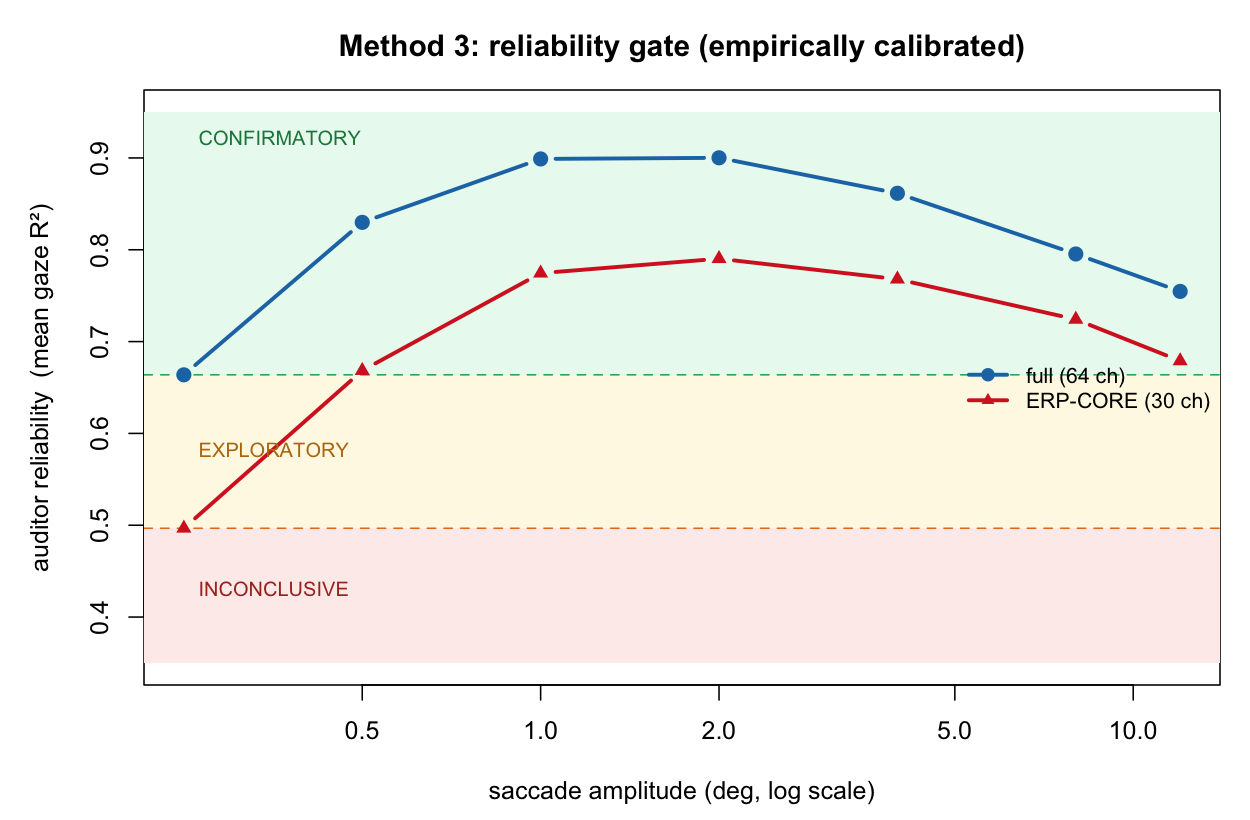
\includegraphics[width=\linewidth]{fig6_reliability_gate.png}
\caption{Reliability gate. The sparse 30-channel ERP-CORE subset drops into the exploratory zone
at the fixational extreme, while the full 64-channel montage stays confirmatory
throughout.}\label{fig:gate}
\end{figure}

\subsection{Neural leakage is bounded by a measurable angle}

Sweeping a lateralized neural source from posterior to frontal with \emph{no} ocular
coupling---so any positive OPI is pure leakage---the leakage is governed by the overlap $s$ of
Eq.~\eqref{eq:overlap} (Fig.~\ref{fig:leak}). It rises monotonically with $s$ (Spearman
$\rho=0.95$ across the swept range), from $+0.006$ at near-orthogonality ($s\approx0.02$, the
posterior-N2pc regime) to $+0.12$--$0.14$ when the source is frontal ($s\approx0.6$--$0.8$). The
headline posterior case is thus low-leakage under the linear model, and any target with a frontal
cognitive topography is flagged by a large $s$ for the leakage-corrected envelope.

\begin{figure}[tb]
\centering
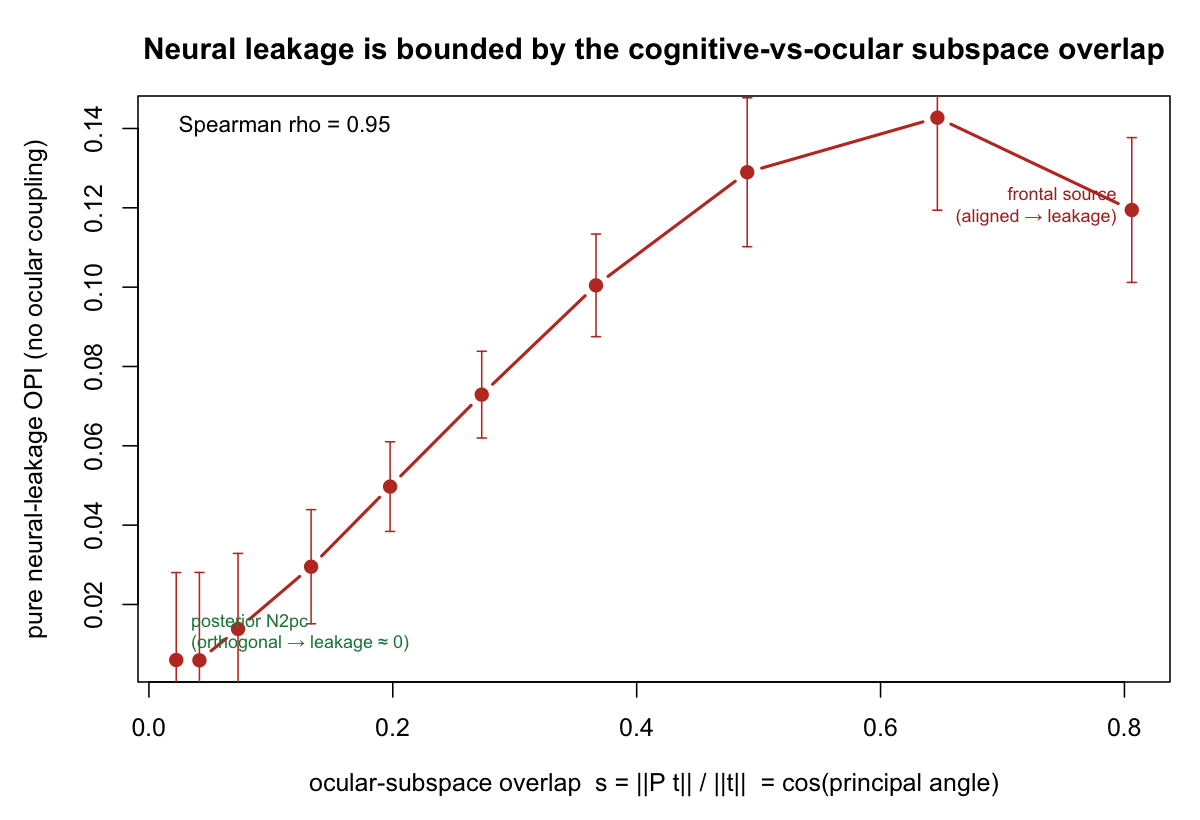
\includegraphics[width=\linewidth]{fig8_leakage_angle.png}
\caption{Neural leakage versus the cognitive-vs-ocular subspace overlap $s=\cos\theta$. Pure
neural-leakage OPI rises monotonically with $s$ ($\rho=0.95$) and is $\approx 0$ for a
posterior (orthogonal) source.}\label{fig:leak}
\end{figure}

\subsection{A headline-analog audit is gated honestly}

To emulate the deployment case we audited a simulated ERP-CORE-like N2pc target on the sparse
montage carrying a sub-$0.2^\circ$ condition-correlated ocular residual of the kind that
survives strict eye-movement rejection. The OPI was positive and significant (0.150, ceiling
AUC 0.777, $p<0.005$), \emph{but the reliability gate returned ``inconclusive''} ($R^2=0.429$,
below the exploratory threshold). The instrument withholds certification of a positive,
significant index because the montage and regime cannot reconstruct gaze well enough to trust
it---the intended ``inconclusive by design'' safeguard, not a false alarm.

\subsection{Real-EEG negative control}

On real 64-channel \texttt{eegmmidb} with the ocular subspace frozen from independent subjects'
eyes-open baseline (Table~\ref{tab:real}, Fig.~\ref{fig:real}), the left-versus-right
imagery contrast---where the eyes have no reason to differ---is weakly decodable from full EEG
(AUC 0.601) but not from the ocular subspace (OPI $-0.023$, $p=0.998$): a clean negative control
on real data. The rest-versus-move contrast is included as a cautionary case: a
frontal-channel-proxy subspace (the best obtainable without an eye-tracker) retains frontal
\emph{neural} signal it cannot separate from ocular activity (OPI $+0.114$, $p=0.002$). This is
the empirical argument for the instrument's design: the auditor must be trained on synchronized
gaze, which isolates the ocular subspace from frontal neural activity, rather than on channel
proxies.

\begin{table}[tb]
\centering
\caption{Real-EEG audit (\texttt{eegmmidb}; ocular subspace frozen from source subjects'
eyes-open baseline; subject-wise evaluation).}\label{tab:real}
\begin{threeparttable}
{\small
\begin{tabular*}{\columnwidth}{@{\extracolsep{\fill}} l cccc @{}}
\toprule
\textbf{Contrast} & \textbf{ceiling} & \textbf{proj} & \textbf{OPI} & \textbf{$p$} \\
\midrule
Left vs.\ right imagery\tnote{a} & 0.601 & 0.501 & $-0.023$ & 0.998 \\
Rest vs.\ move\tnote{b}          & 0.672 & 0.615 & $+0.114$ & 0.002 \\
\bottomrule
\end{tabular*}}
\begin{tablenotes}
\small
\item[a] Clean negative control (no differential gaze): not decodable from the ocular subspace.
\item[b] Cautionary: a no-eye-tracker channel proxy retains frontal neural signal.
\end{tablenotes}
\end{threeparttable}
\end{table}

\begin{figure}[tb]
\centering
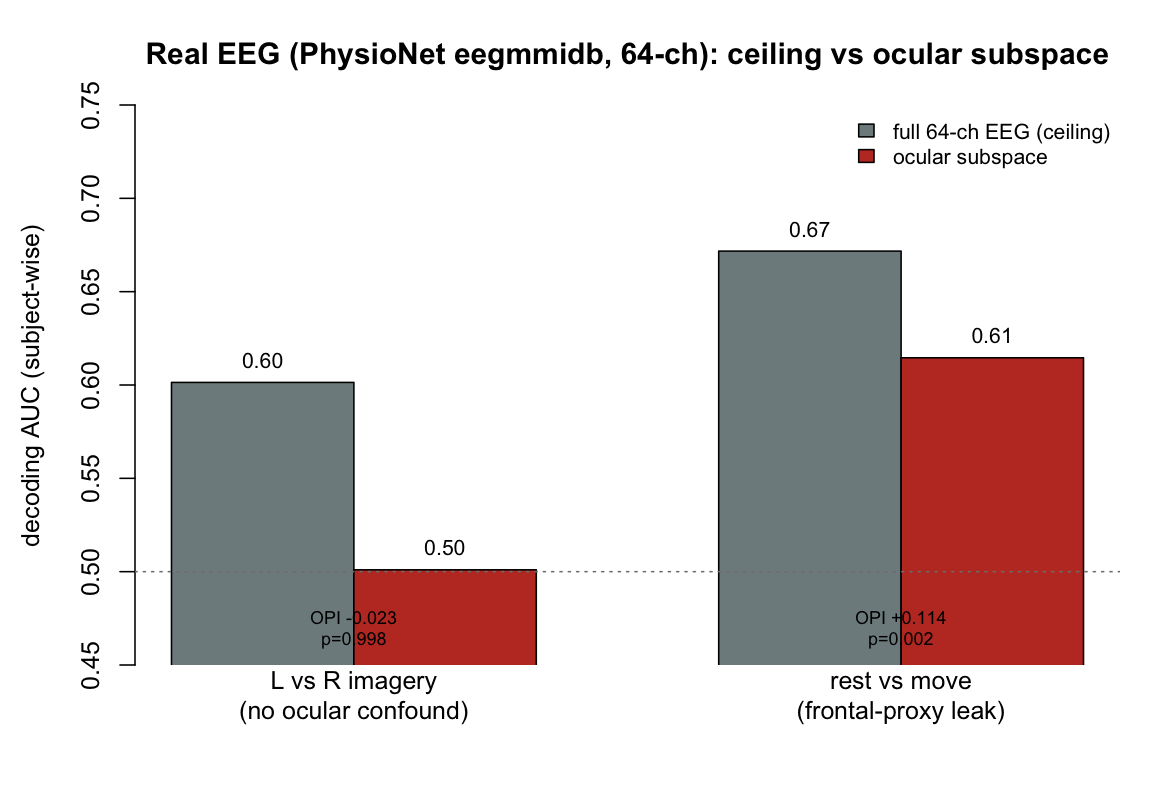
\includegraphics[width=\linewidth]{fig7_real_eegmmidb.png}
\caption{Real EEG (\texttt{eegmmidb}). Full-EEG ceiling (grey) versus ocular-subspace (red)
decoding AUC. Left-versus-right imagery is at chance in the ocular subspace; rest-versus-move
leaks through the channel proxy.}\label{fig:real}
\end{figure}

%%──────────────────────────────────────────────────────────
%% DISCUSSION
%%──────────────────────────────────────────────────────────

\section{Discussion}\label{sec:discussion}

We have defined a frozen, montage-matched ocular-subspace auditor and shown, against ground
truth, that it does what an audit instrument must: it is sensitive to more than one artifact
type (OPI 0.43 for saccade-coupled and 0.20 for blink-coupled contamination), specific
(near-null on neural and shuffled controls), graded (monotone in the coupling), conservative
(a measured, signed bias envelope that errs toward under-stating), self-aware (a reliability
gate that returns ``inconclusive''), and---critically---honest about its one residual failure
mode, neural leakage, which we render as a computable number, the principal-angle overlap $s$.
Throughout, the auditor uses all 64 channels; the 30-channel ERP-CORE case is reported as an
explicit subset to quantify how channel count affects reliability, not as a hidden reduction.

\emph{Relation to prior work.} The instrument generalizes the within-experiment control of
\citet{mostert2018eye} and the single-domain diagnosis of \citet{rotaru2024decoding} into a
transferable meter that requires no eye-tracker on the target, complementing rather than
replacing ocular removal~\cite{jung2000removing,dimigen2020optimizing} and within-recording
deconvolution~\cite{ehinger2019unfold}. Where confound-quantification in machine learning
probes a \emph{measured} nuisance variable~\cite{chaibubneto2018permutations}, here the nuisance
(gaze) is \emph{physically recovered} even when it was never recorded in the target, and the
back-door through which it could mislead---neural leakage---is bounded by Eq.~\eqref{eq:overlap}.
This positions the work in the now-active genre of auditing the field's results for inflated
inference~\cite{eklund2016cluster,kapoor2023leakage,brookshire2024leakage}.

\emph{Toward a field-wide audit.} Because the instrument is portable and CPU-cheap, the natural
deployment is an ocular-leakage audit across widely used public benchmarks---community-trusted
ERP data~\cite{kappenman2021erpcore}, P300~\cite{polich2007p300} spellers including overt/covert
designs~\cite{arico2014p300jitter,korczowski2019bi2015a}, rapid visual streams without any
eye-tracker~\cite{gifford2022thingseeg2}, and motor-imagery sets, accessed
uniformly via MOABB~\cite{jayaram2018moabb}---each no-eye-tracker benchmark paired with a
gaze- or EOG-bearing anchor so that verdicts are ground-truthable. The competence boundary makes
such a leaderboard honest: a benchmark on which gaze cannot be reconstructed is reported
``inconclusive,'' not falsely cleared.

\subsection{Limitations}

The ground-truth validation is necessarily simulation-based, because measuring bias requires
knowing the true ocular contribution; the simulator is grounded in measured physiology but is a
simplification (notably, spatial features rather than full spatiotemporal windows, and a linear
generative structure aligned with the linear operator). The leakage bound $s$ upper-bounds the
overlap and its monotonic relationship to leakage is shown empirically under the linear-subspace
model; both should be tested across real cognitive topographies. Real synchronized-gaze datasets
such as EEGEyeNet~\cite{kastrati2021eegeyenet} and ZuCo~\cite{hollenstein2018zuco,hollenstein2020zuco2}
are the appropriate anchors for training the readout and validating verdicts, but their training
paradigms are cued large saccades, so the sub-degree fixational regime must be anchored on
reading microsaccades rather than assumed. The real-EEG demonstration used a channel-proxy
subspace because \texttt{eegmmidb} has no eye-tracker; it therefore validates the negative-control
logic and the design rationale, not a gaze-trained transfer. Finally, the index measures only the
ocular subspace; it will not detect non-ocular confounds such as repeated-stimulus fingerprints.

%%──────────────────────────────────────────────────────────
%% CONCLUSIONS
%%──────────────────────────────────────────────────────────

\section{Conclusions}

How much of an EEG decoding result could be the eyes rather than the mind is, for most published
datasets, an unanswerable question because no eye-tracker was present. A frozen, montage-matched
ocular-subspace auditor makes it answerable: it converts the worry into a calibrated, two-sided
Ocular Predictability Index with a self-declared competence boundary and a computable
neural-leakage bound, validated here against ground truth and demonstrated on real EEG. The
instrument is small, CPU-runnable, and released, and it is built to be pointed at the field's
benchmarks---reporting ``inconclusive'' wherever it honestly cannot see.

%%──────────────────────────────────────────────────────────
%% DECLARATIONS
%%──────────────────────────────────────────────────────────

\section*{Declarations}

\noindent\textbf{Ethics approval and consent to participate}\\
Not applicable. This study analyzed only publicly available, de-identified datasets and
synthetic data; it involved no new human-subjects data collection.

\smallskip
\noindent\textbf{Consent for publication}\\
Not applicable.

\smallskip
\noindent\textbf{Availability of data and materials}\\
All datasets are publicly available: EEGEyeNet (\url{https://osf.io/ktv7m/}), ERP~CORE
(\url{https://erpinfo.org/erp-core}), ZuCo (\url{https://osf.io/q3zws/},
\url{https://osf.io/2urht/}), PhysioNet \texttt{eegmmidb}
(\url{https://physionet.org/content/eegmmidb/}), and Brain Invaders (Zenodo). The auditor
implementation, simulator, and all analysis code and result tables are released with this article.

\smallskip
\noindent\textbf{Competing interests}\\
The authors declare that they have no competing interests.

\smallskip
\noindent\textbf{Funding}\\
This research received no specific external funding.

\smallskip
\noindent\textbf{Authors' contributions}\\
Not applicable (author information withheld).

\smallskip
\noindent\textbf{Acknowledgements}\\
The authors thank the providers of the open datasets used in this work.

%%──────────────────────────────────────────────────────────
%% ABBREVIATIONS
%%──────────────────────────────────────────────────────────

\section*{List of Abbreviations}

\noindent\textbf{AUC:} Area under the receiver operating characteristic curve\\
\textbf{EEG:} Electroencephalography\\
\textbf{EOG:} Electrooculography\\
\textbf{HEOG:} Horizontal electrooculogram\\
\textbf{ICA:} Independent component analysis\\
\textbf{OPI:} Ocular Predictability Index\\
\textbf{N2pc:} N2-posterior-contralateral component\\
\textbf{VEOG:} Vertical electrooculogram

%%──────────────────────────────────────────────────────────
%% REFERENCES
%%──────────────────────────────────────────────────────────

\bibliographystyle{unsrtnat}
\bibliography{sn-bibliography}

\end{document}
